% =====================================================================
%  Rapport technique - Projet Machine Learning I (EFREI 2026-2027)
%  Classification de la qualité du vin
%  Compilation : pdflatex rapport_projet_vin.tex (deux fois, pour la table des matières)
%  Les figures sont dans le dossier fig/ (exportées du notebook projet\_vin.ipynb)
% =====================================================================
\documentclass[11pt,a4paper]{article}

\usepackage[T1]{fontenc}
\usepackage[utf8]{inputenc}
\usepackage{lmodern}
\usepackage[french]{babel}
\usepackage[a4paper,margin=2.4cm]{geometry}
\usepackage{microtype}
\usepackage{amsmath,amssymb}
\usepackage{graphicx}
\usepackage{booktabs}
\usepackage{multirow}
\usepackage{makecell}
\usepackage{float}
\usepackage[font=small,labelfont=bf]{caption}
\usepackage{subcaption}
\usepackage{xcolor}
\usepackage{enumitem}
\usepackage{fancyhdr}
\usepackage[ruled,vlined,linesnumbered,french]{algorithm2e}
\usepackage{tikz}
\usetikzlibrary{arrows.meta,positioning}
\usepackage[hidelinks]{hyperref}
\usepackage{csquotes}

\graphicspath{{fig/}}
\definecolor{vin}{RGB}{122,31,43}
\setlist{itemsep=2pt,topsep=4pt}

\pagestyle{fancy}
\fancyhf{}
\lhead{\small Machine Learning I -- Projet}
\rhead{\small Classification de la qualité du vin}
\cfoot{\thepage}
\renewcommand{\headrulewidth}{0.4pt}

\newcommand{\code}[1]{\texttt{#1}}
\newcommand{\Fun}{F_1}

% ---------------------------------------------------------------------
\begin{document}

% ============================ Page de titre ===========================
\begin{titlepage}
  \centering
  {\large EFREI Paris -- Cycle ingénieur\par}
  {\large Machine Learning I \quad -- \quad Année 2026--2027\par}
  \vspace{3.2cm}
  {\color{vin}\rule{\linewidth}{1pt}\par}
  \vspace{0.6cm}
  {\Huge\bfseries Classification de la qualité du vin\par}
  \vspace{0.4cm}
  {\Large à partir de ses propriétés physico-chimiques\par}
  \vspace{0.6cm}
  {\color{vin}\rule{\linewidth}{1pt}\par}
  \vspace{1cm}
  {\Large Rapport technique\par}
  \vfill
  \begin{tabular}{rl}
    \textbf{Auteurs :} & \textit{[Nom Prénom]} \\
                       & \textit{[Nom Prénom]} \\
                       & \textit{[Nom Prénom]} \\[6pt]
    \textbf{Encadrants :} & Ahmed Ghazi \textsc{Blaiech}, Ahmad \textsc{Tay}, Hassan \textsc{Shraim} \\
  \end{tabular}
  \vspace{1.5cm}

  {\small Code : notebook \code{projet\_vin.ipynb} (Python, scikit-learn)\par}
\end{titlepage}

% ============================== Résumé ================================
\begin{abstract}
\noindent
Ce rapport présente une chaîne complète d'apprentissage supervisé visant à prédire si un vin est \og bon \fg{} (note d'experts $\geq 7$) à partir de onze mesures physico-chimiques. Les données proviennent du jeu \emph{Wine Quality} de l'UCI (vins rouges et blancs portugais \emph{Vinho Verde}). Après nettoyage (suppression de 1\,177 doublons, détection des valeurs aberrantes par la règle de Tukey, encodage), nous obtenons 5\,320 vins, dont seulement 19\,\% de \og bons \fg{}. Ce fort déséquilibre guide l'ensemble des choix méthodologiques : découpage stratifié, pondération des classes et utilisation du score $\Fun$ et de l'AUC plutôt que de l'exactitude. Une sélection de variables par élimination récursive (RFE) confirme le rôle dominant du degré d'alcool et de l'acidité volatile. Cinq classifieurs sont comparés (régression logistique, $k$ plus proches voisins, arbre de décision, Naive Bayes gaussien, SVM à noyau RBF), d'abord par validation croisée à 5 plis sur l'ensemble d'apprentissage, avec un diagnostic biais/variance, puis après optimisation de leurs hyperparamètres par recherche en grille et recherche aléatoire. Le jeu de test n'est utilisé qu'une seule fois, pour l'évaluation finale. Le SVM à noyau RBF obtient les meilleures performances ($\Fun = 0{,}54$, AUC $= 0{,}85$, rappel $= 0{,}82$ sur le test) et le meilleur compromis biais/variance. Les performances, modestes en valeur absolue, sont discutées au regard de la subjectivité de la note et du chevauchement des classes.
\end{abstract}

\vspace{0.5cm}
\tableofcontents
\newpage

% ============================ 1. Introduction =========================
\section{Introduction}

\subsection{Contexte}
La qualité d'un vin est traditionnellement évaluée par des dégustateurs experts, ce qui est coûteux, lent et en partie subjectif. Or de nombreuses grandeurs physico-chimiques (acidité, sucre résiduel, teneur en alcool, sulfites, etc.) sont mesurées en routine lors de la certification. La question est donc de savoir si ces mesures objectives suffisent à prédire le jugement des experts. Aucune formule analytique ne relie ces mesures à la qualité perçue : c'est un cas typique où l'apprentissage automatique permet d'extraire une règle de décision à partir d'exemples étiquetés.

\subsection{Problématique et objectifs}
Conformément au sujet, le problème initialement ordinal (note de 0 à 10) est reformulé en \textbf{classification binaire} : un vin est \og bon \fg{} si sa note est supérieure ou égale à 7, \og pas bon \fg{} sinon. Les objectifs sont :
\begin{enumerate}
  \item préparer et analyser les données (qualité, distributions, corrélations, équilibre des classes) ;
  \item sélectionner les variables pertinentes avec une méthode vue en cours ;
  \item comparer cinq modèles de natures différentes (linéaire / non linéaire, paramétrique / non paramétrique, probabiliste / géométrique) ;
  \item évaluer ces modèles avec des métriques adaptées au déséquilibre et identifier le meilleur compromis biais/variance ;
  \item optimiser leurs hyperparamètres et mesurer la performance finale sur des données jamais vues.
\end{enumerate}

\subsection{Organisation du rapport}
La section~\ref{sec:donnees} décrit les données et la section~\ref{sec:pretraitement} leur prétraitement. La section~\ref{sec:cible} définit la cible et traite le déséquilibre des classes, puis la section~\ref{sec:eda} présente l'analyse exploratoire. Le protocole expérimental est détaillé en section~\ref{sec:protocole} et la sélection de variables en section~\ref{sec:selection}. Les sections~\ref{sec:modeles} à~\ref{sec:final} portent sur les modèles, leur évaluation, leur optimisation et l'évaluation finale. La section~\ref{sec:discussion} discute les limites et perspectives.

% ============================ 2. Données ==============================
\section{Données}\label{sec:donnees}

Nous utilisons le jeu de données \emph{Wine Quality} de l'UCI Machine Learning Repository~\cite{cortez2009}, composé de deux fichiers : 1\,599 vins rouges et 4\,898 vins blancs, soit 6\,497 observations. Chaque vin est décrit par onze variables continues issues de tests physico-chimiques et par une note médiane attribuée par au moins trois experts (tableau~\ref{tab:variables}). Les notes observées vont de 3 à 9.

\begin{table}[H]
\centering
\caption{Variables du jeu de données.}
\label{tab:variables}
\small
\begin{tabular}{lll}
\toprule
\textbf{Variable} & \textbf{Description} & \textbf{Unité} \\
\midrule
\code{fixed acidity}        & acidité fixe (acide tartrique)        & g/L \\
\code{volatile acidity}     & acidité volatile (acide acétique)      & g/L \\
\code{citric acid}          & acide citrique                         & g/L \\
\code{residual sugar}       & sucre résiduel                         & g/L \\
\code{chlorides}            & chlorures (sel)                        & g/L \\
\code{free sulfur dioxide}  & SO$_2$ libre                           & mg/L \\
\code{total sulfur dioxide} & SO$_2$ total                           & mg/L \\
\code{density}              & densité                                & g/cm$^3$ \\
\code{pH}                   & pH                                     & -- \\
\code{sulphates}            & sulfates                               & g/L \\
\code{alcohol}              & teneur en alcool                       & \% vol. \\
\midrule
\code{type}                 & couleur (ajoutée lors de la fusion)    & rouge / blanc \\
\code{quality}              & note des experts                       & 0 à 10 \\
\bottomrule
\end{tabular}
\end{table}

Les deux fichiers ont été fusionnés afin de disposer de davantage d'exemples, en particulier pour les vins rouges, moins nombreux. Une variable \code{type} conserve l'information de couleur, ce qui permet au modèle de l'exploiter si elle est utile. Les statistiques descriptives révèlent deux points importants pour la suite : (i) des échelles très hétérogènes (densité proche de 1, SO$_2$ total jusqu'à 440 mg/L), qui imposent une standardisation pour les méthodes fondées sur des distances ; (ii) des maxima très éloignés du troisième quartile pour plusieurs variables (\code{residual sugar}, \code{chlorides}, \code{free sulfur dioxide}), signe de valeurs extrêmes.

% ========================== 3. Prétraitement ==========================
\section{Prétraitement}\label{sec:pretraitement}

\subsection{Valeurs manquantes et doublons}
Aucune valeur manquante n'est présente : aucune imputation n'est nécessaire. En revanche, le jeu contient \textbf{1\,177 doublons exacts} (18\,\% des lignes), soit exactement la somme des doublons internes à chaque fichier (240 rouges et 937 blancs) : la fusion n'en crée aucun. Ces doublons sont supprimés \emph{avant} le découpage apprentissage/test. Sans cette précaution, deux copies d'un même vin pourraient se retrouver de part et d'autre du découpage, et le modèle serait évalué sur des exemples déjà vus, ce qui gonflerait artificiellement les scores. Il reste \textbf{5\,320 vins}.

\subsection{Valeurs aberrantes}
Les valeurs aberrantes sont détectées par la règle de Tukey~\cite{tukey1977}, qui définit les moustaches d'une boîte à moustaches. Avec $Q_1$ et $Q_3$ les premier et troisième quartiles et $\mathrm{IQR} = Q_3 - Q_1$ l'écart interquartile, une valeur $x$ est signalée si
\begin{equation}
x < Q_1 - 1{,}5\,\mathrm{IQR} \quad \text{ou} \quad x > Q_3 + 1{,}5\,\mathrm{IQR}.
\end{equation}
Fondée sur les quartiles, cette règle est robuste : les valeurs extrêmes ne déplacent pas les bornes, contrairement à un critère fondé sur la moyenne et l'écart-type. Elle ne suppose pas non plus de distribution gaussienne, hypothèse non vérifiée ici.

Les vins rouges et blancs ayant des compositions chimiques différentes, l'IQR a été recalculé \emph{séparément pour chaque couleur} (figure~\ref{fig:outliers}). Le nombre total de valeurs signalées varie peu (environ 1\,370 sur le jeu mélangé contre 1\,340 par couleur), mais sa répartition change nettement. Pour \code{fixed acidity} et \code{volatile acidity}, le nombre de valeurs signalées est divisé par deux environ (304 $\to$ 147 et 279 $\to$ 152) : une partie de ces \og anomalies \fg{} ne traduisait que l'écart entre rouges et blancs. À l'inverse, le mélange masquait des valeurs atypiques pour \code{density} (3 $\to$ 41) ou \code{total sulfur dioxide} (10 $\to$ 59).

\begin{figure}[H]
\centering
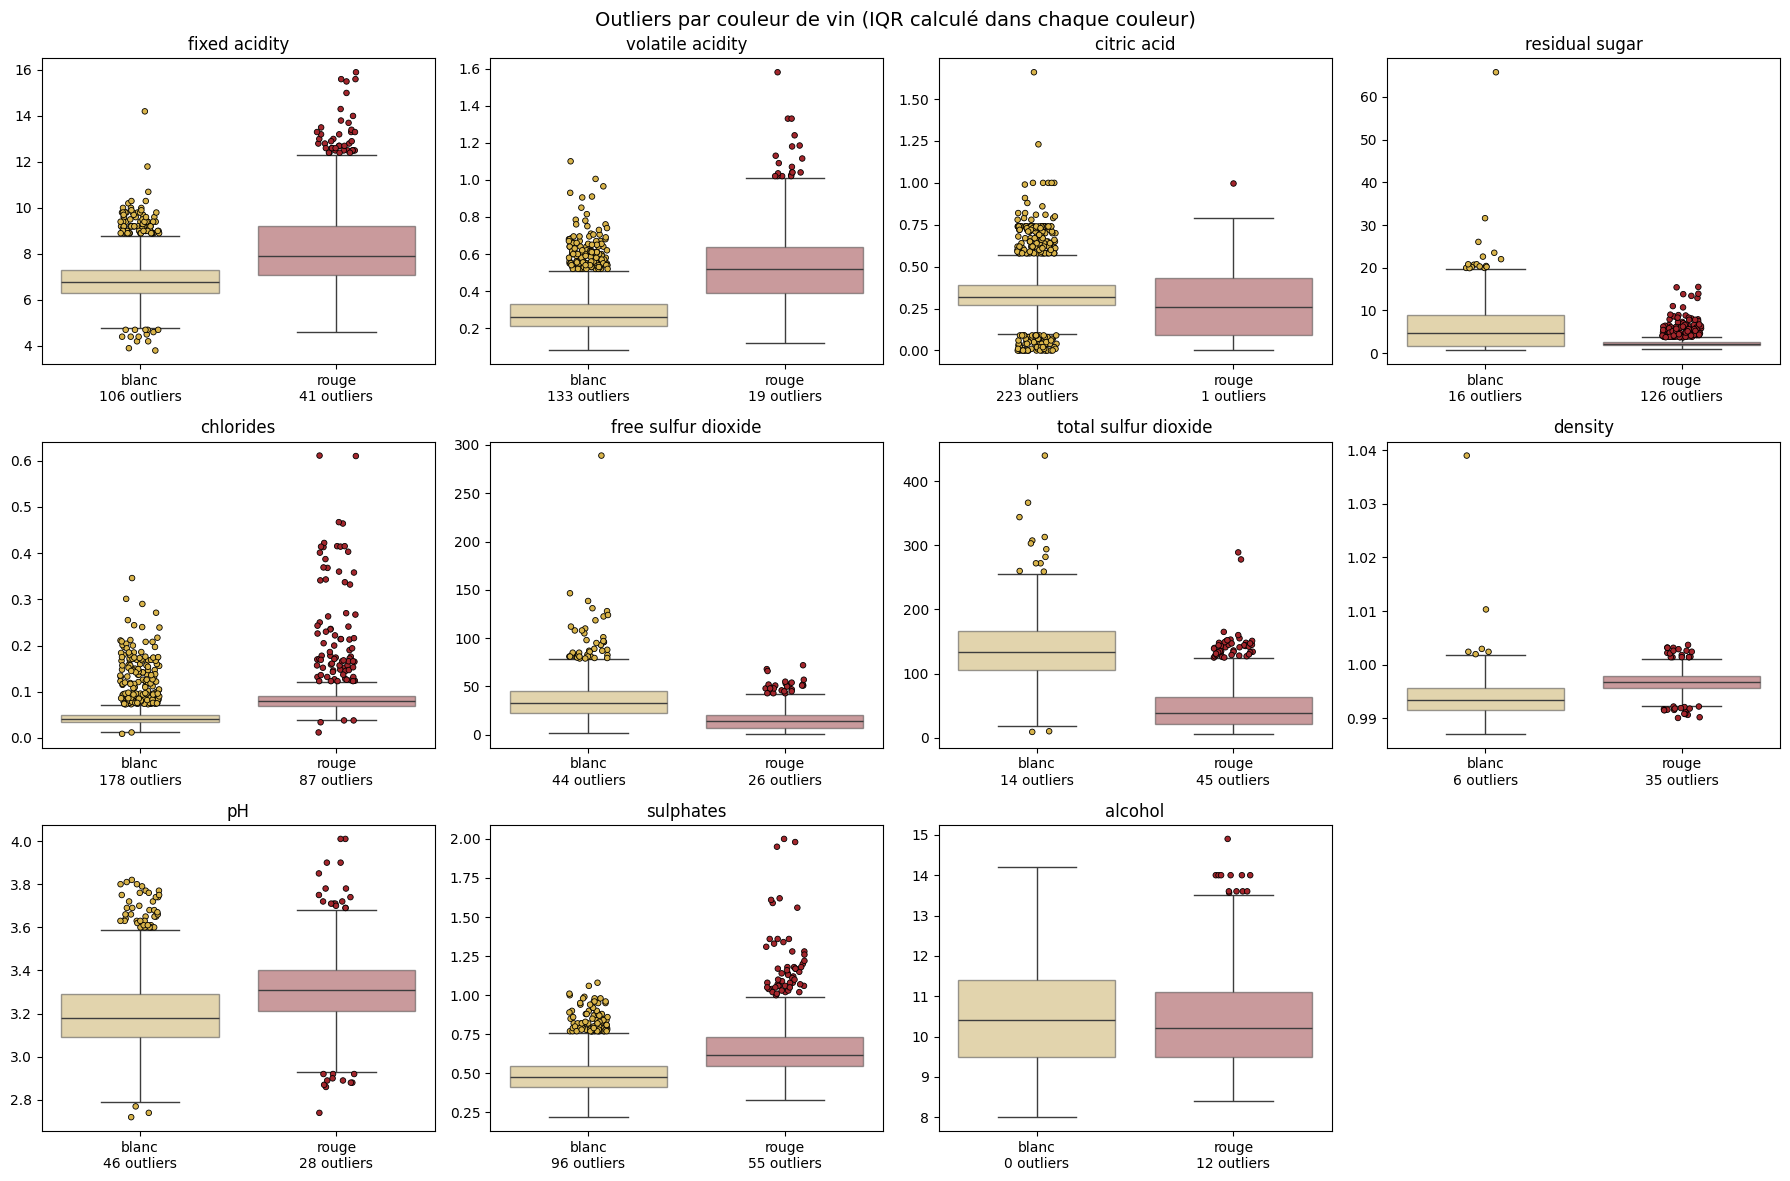
\includegraphics[width=0.92\linewidth]{outliers_couleur.png}
\caption{Valeurs aberrantes détectées par la règle de Tukey, calculée séparément pour les vins blancs et rouges.}
\label{fig:outliers}
\end{figure}

Dans chaque couleur, les valeurs signalées représentent le plus souvent 1 à 6\,\% des vins et forment des queues continues de distribution, ce qui correspond à des vins atypiques plutôt qu'à des erreurs de mesure. Le taux élevé observé pour le sucre résiduel des rouges (9{,}3\,\%) s'explique par une distribution très resserrée autour de 2~g/L, qui rend la règle très stricte ; les valeurs signalées (4 à 15~g/L) restent plausibles. Nous avons donc \textbf{conservé toutes les observations}, leur influence étant limitée par la standardisation (section~\ref{sec:protocole}).

\subsection{Encodage}
La variable \code{type} est la seule variable catégorielle. Ayant deux modalités sans ordre, elle est codée en binaire (blanc~$=0$, rouge~$=1$). Un encodage \emph{one-hot} produirait deux colonnes parfaitement redondantes.

% ====================== 4. Cible et déséquilibre ======================
\section{Variable cible et déséquilibre des classes}\label{sec:cible}

La cible est définie par $y = \mathbb{1}[\code{quality} \geq 7]$. Elle est fortement déséquilibrée : \textbf{81\,\% de vins \og pas bons \fg{} et 19\,\% de \og bons \fg{}} (figure~\ref{fig:cible}).

\begin{figure}[H]
\centering
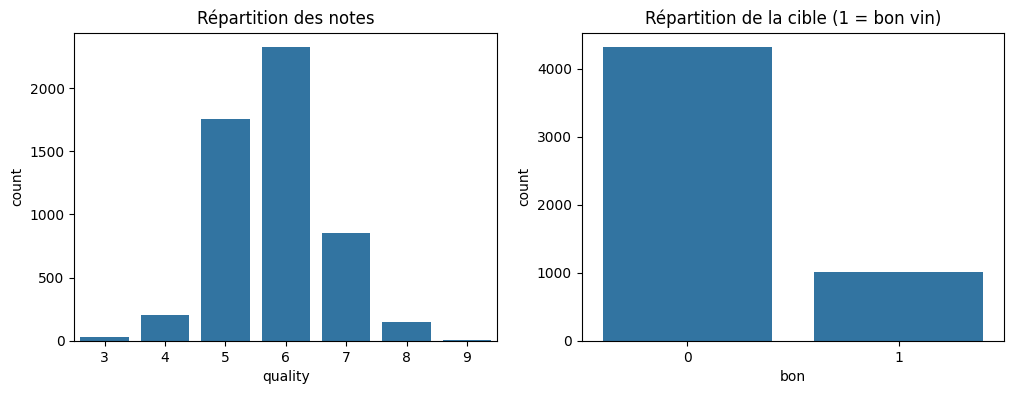
\includegraphics[width=0.85\linewidth]{cible.png}
\caption{Répartition des notes (gauche) et de la cible binaire (droite).}
\label{fig:cible}
\end{figure}

Ce déséquilibre rend l'exactitude (\emph{accuracy}) trompeuse : un classifieur trivial prédisant toujours \og pas bon \fg{} atteindrait 81\,\% d'exactitude sans détecter aucun bon vin. Trois mesures ont été prises.
\begin{itemize}
  \item \textbf{Découpage stratifié} : les ensembles d'apprentissage et de test conservent la proportion de 19\,\% de bons vins.
  \item \textbf{Pondération des classes} (\code{class\_weight="balanced"}), lorsque le modèle le permet. Le poids de la classe $c$ vaut
  \begin{equation}
    w_c = \frac{n}{K\, n_c},
  \end{equation}
  où $n$ est le nombre d'exemples, $K=2$ le nombre de classes et $n_c$ l'effectif de la classe. Sur l'ensemble d'apprentissage ($n = 4\,256$, dont 807 bons vins), on obtient $w_{\text{bon}} \approx 2{,}64$ et $w_{\text{pas bon}} \approx 0{,}62$ : une erreur sur un bon vin coûte environ quatre fois plus cher. C'est le même principe que la pondération des observations dans AdaBoost.
  \item \textbf{Métriques adaptées} : le score $\Fun$ de la classe positive est la métrique principale, complétée par l'AUC, indépendante du seuil de décision (section~\ref{sec:evaluation}).
\end{itemize}
Une alternative, discutée en section~\ref{sec:discussion}, consiste à conserver un apprentissage non pondéré et à ajuster le seuil de décision à partir de la courbe ROC.

% =================== 5. Analyse exploratoire ==========================
\section{Analyse exploratoire}\label{sec:eda}

\paragraph{Distributions.} Les histogrammes montrent que plusieurs variables (\code{chlorides}, \code{residual sugar}, \code{sulphates}) sont fortement asymétriques à droite. L'hypothèse gaussienne du classifieur Naive Bayes est donc violée, ce qui laisse prévoir des performances moindres pour ce modèle.

\paragraph{Corrélations.} Le coefficient de corrélation de Pearson entre chaque variable et la cible place nettement en tête l'alcool ($r = +0{,}42$), suivi de la densité ($-0{,}29$), des chlorures ($-0{,}16$) et de l'acidité volatile ($-0{,}14$) ; toutes les autres variables ont $|r| < 0{,}09$. Plusieurs variables explicatives sont fortement corrélées entre elles : SO$_2$ libre et total ($0{,}72$), densité et alcool ($-0{,}67$), densité et sucre résiduel ($0{,}52$). Ces dépendances sont physiquement attendues (la densité d'un vin dépend de sa teneur en alcool et en sucre) et violent l'hypothèse d'indépendance de Naive Bayes.

\begin{figure}[H]
\centering
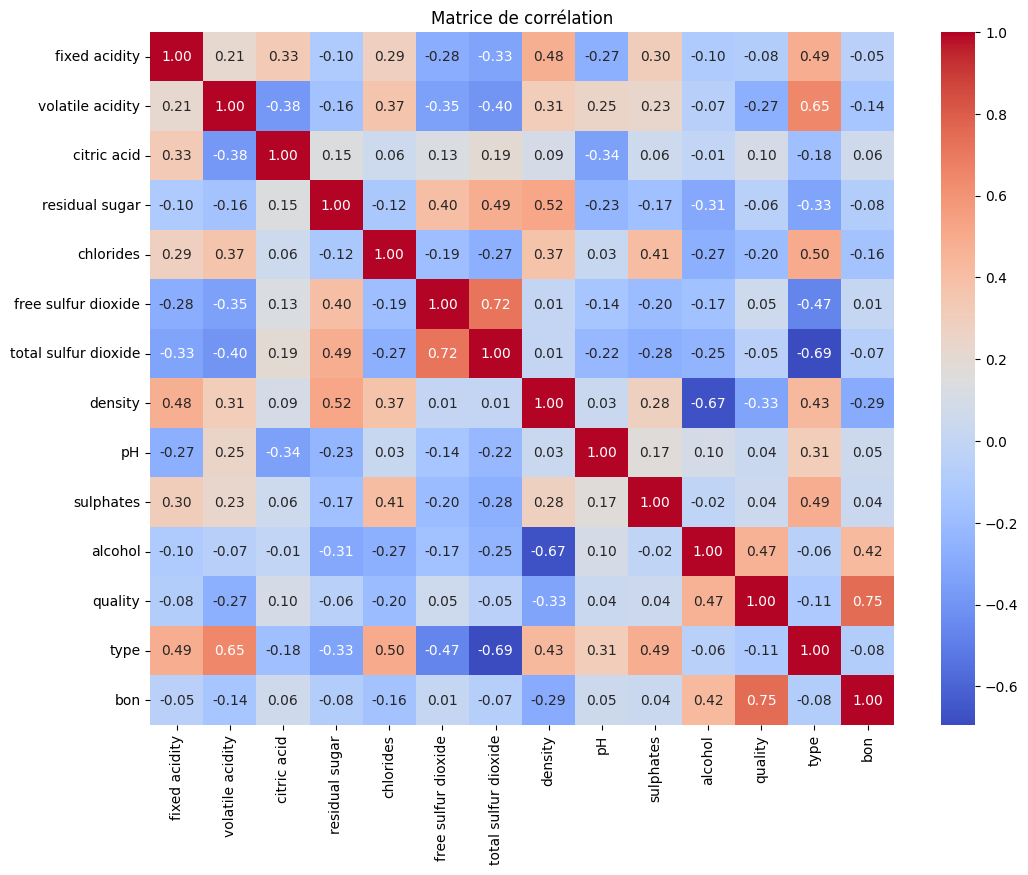
\includegraphics[width=0.62\linewidth]{correlation.png}
\caption{Matrice des corrélations de Pearson (variables explicatives, note et cible).}
\label{fig:corr}
\end{figure}

\paragraph{Boîtes à moustaches par classe.} Pour les quatre variables les plus corrélées à la cible (figure~\ref{fig:boxclasse}), les bons vins présentent une teneur en alcool nettement plus élevée, ainsi qu'une densité, une acidité volatile et une teneur en chlorures plus faibles. L'alcool est la variable qui sépare le mieux les deux classes. Ces observations sont cohérentes avec l'œnologie : l'acidité volatile, principalement due à l'acide acétique, est un défaut gustatif classique.

\begin{figure}[H]
\centering
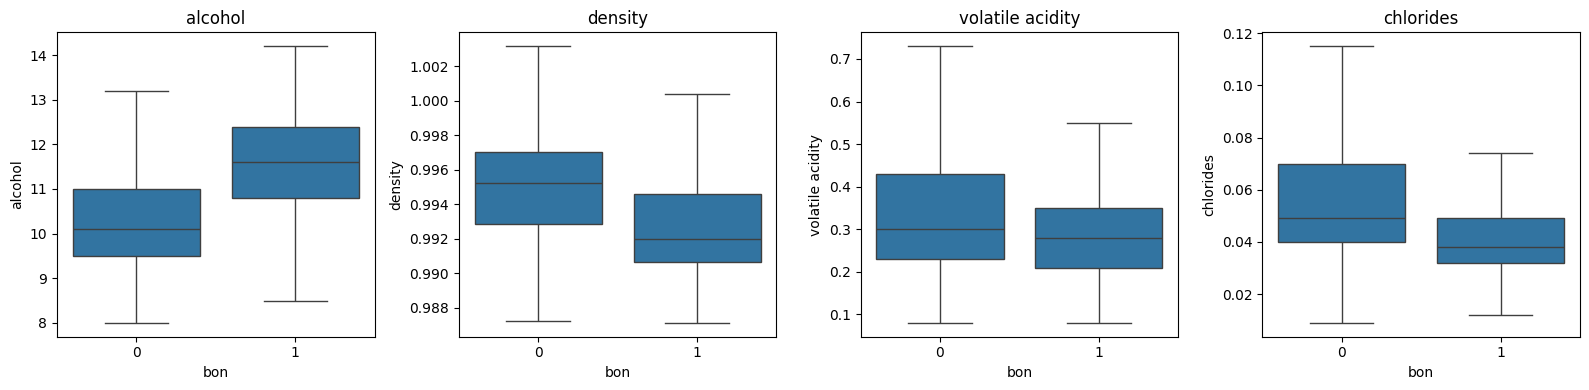
\includegraphics[width=\linewidth]{boxplots_classe.png}
\caption{Distribution des quatre variables les plus corrélées à la cible, selon la classe (0 = pas bon, 1 = bon).}
\label{fig:boxclasse}
\end{figure}

% ===================== 6. Protocole expérimental =======================
\section{Protocole expérimental}\label{sec:protocole}

\subsection{Découpage et standardisation}
Les données sont découpées en un ensemble d'apprentissage (80\,\%, 4\,256 vins dont 807 bons) et un ensemble de test (20\,\%, 1\,064 vins dont 202 bons), de façon stratifiée et reproductible (\code{random\_state=42}). Les variables sont ensuite standardisées (\emph{z-score}) :
\begin{equation}
z_j = \frac{x_j - \mu_j}{\sigma_j},
\end{equation}
où $\mu_j$ et $\sigma_j$ sont la moyenne et l'écart-type de la variable $j$ \textbf{calculés sur l'ensemble d'apprentissage uniquement}, puis appliqués tels quels au test. La standardisation est préférée à la normalisation min-max car les variables ont des unités très différentes, et parce que la normalisation min-max dépend des valeurs extrêmes (un sucre résiduel de 66~g/L comprimerait tous les autres vins).

\subsection{Validation croisée et usage unique du test}
Toute décision (sélection de variables, choix des hyperparamètres, choix du modèle) est prise par \textbf{validation croisée stratifiée à 5 plis sur l'ensemble d'apprentissage}. Pour les tableaux de résultats, matrices de confusion et courbes ROC des modèles par défaut, nous utilisons des prédictions \emph{hors-pli} (\emph{out-of-fold}) : chaque vin de l'apprentissage est prédit par un modèle entraîné sur les quatre autres plis, qui ne l'a donc jamais vu. Le \textbf{jeu de test n'est utilisé qu'une seule fois}, pour l'évaluation finale des modèles optimisés. Utiliser le test pour choisir un modèle reviendrait à l'optimiser pour cet échantillon particulier, et le score obtenu ne serait plus une estimation non biaisée de l'erreur de généralisation. La figure~\ref{fig:pipeline} résume ce protocole.

\begin{figure}[H]
\centering
\begin{tikzpicture}[
  node distance=0.5cm and 0.45cm,
  box/.style={draw=vin, rounded corners=2pt, fill=vin!6, align=center, font=\small, minimum height=1cm, text width=2.35cm},
  test/.style={draw=black!60, rounded corners=2pt, fill=black!6, align=center, font=\small, minimum height=1cm, text width=2.35cm},
  arr/.style={-{Latex[length=2mm]}, thick, vin}]
  \node[box] (a) {Données nettoyées\\(5\,320 vins)};
  \node[box, right=of a] (b) {Découpage stratifié\\80\,/\,20};
  \node[box, right=of b] (c) {Standardisation\\(fit sur train)};
  \node[box, right=of c] (d) {RFE\\+ CV 5 plis};
  \node[box, below=0.9cm of d] (e) {5 modèles\\défaut : CV};
  \node[box, left=of e] (f) {Diagnostic\\biais / variance};
  \node[box, left=of f] (g) {Grid / Random\\Search (CV)};
  \node[test, left=of g] (h) {\textbf{Test}\\(une seule fois)};
  \draw[arr] (a) -- (b); \draw[arr] (b) -- (c); \draw[arr] (c) -- (d);
  \draw[arr] (d) -- (e); \draw[arr] (e) -- (f); \draw[arr] (f) -- (g); \draw[arr] (g) -- (h);
\end{tikzpicture}
\caption{Protocole expérimental. Toutes les étapes en rouge n'utilisent que l'ensemble d'apprentissage.}
\label{fig:pipeline}
\end{figure}

% ===================== 7. Sélection de variables =======================
\section{Sélection de variables}\label{sec:selection}

\subsection{Méthode : élimination récursive (RFE)}
Parmi les trois familles de méthodes de sélection (filtre, \emph{wrapper}, embarquée), nous retenons une méthode \emph{wrapper}, l'élimination récursive de variables (RFE, algorithme~\ref{alg:rfe}). Contrairement à un filtre, qui évalue chaque variable isolément, la RFE évalue les variables \emph{conjointement} au sein d'un modèle. Elle tient donc compte des redondances et des effets de combinaison. L'estimateur sous-jacent est une régression logistique pondérée (\code{class\_weight="balanced"}) entraînée sur les données standardisées ; l'importance d'une variable est mesurée par la valeur absolue de son coefficient.

\begin{algorithm}[H]
\caption{Élimination récursive de variables (RFE)}
\label{alg:rfe}
\KwIn{ensemble de variables $S = \{1,\dots,p\}$, données d'apprentissage}
\KwOut{rang de chaque variable}
$r \leftarrow p$\;
\While{$|S| > 1$}{
  entraîner une régression logistique sur les variables de $S$\;
  $j^\star \leftarrow \arg\min_{j\in S} |\beta_j|$ \tcp*{variable la moins utile}
  $\text{rang}(j^\star) \leftarrow r$ ; \quad $S \leftarrow S \setminus \{j^\star\}$ ; \quad $r \leftarrow r-1$\;
}
$\text{rang}(\text{dernière variable restante}) \leftarrow 1$\;
\end{algorithm}

\subsection{Résultats}
Le classement obtenu figure au tableau~\ref{tab:rfe}. L'alcool est classé premier, en accord avec l'analyse de corrélation, suivi de l'acidité volatile. Plusieurs différences avec le classement par corrélation sont instructives :
\begin{itemize}
  \item la \textbf{densité}, deuxième variable la plus corrélée à la cible, n'est que cinquième : sa forte dépendance à l'alcool et au sucre la rend largement redondante une fois l'alcool présent dans le modèle ;
  \item les \textbf{chlorures}, troisièmes en corrélation, sont dixièmes pour la même raison ;
  \item l'\textbf{acidité fixe} et le \textbf{pH}, peu corrélés à la cible, sont classés troisième et quatrième : ils deviennent informatifs en combinaison avec d'autres variables, ce qu'un filtre univarié ne peut pas détecter.
\end{itemize}
Une limite de ce classement est qu'il repose sur un modèle linéaire : une variable dont l'effet est uniquement non linéaire peut être sous-évaluée.

\begin{table}[H]
\centering
\caption{Classement RFE et corrélation de Pearson avec la cible.}
\label{tab:rfe}
\small
\begin{tabular}{clr@{\hspace{1.2cm}}clr}
\toprule
\textbf{Rang} & \textbf{Variable} & $r$ & \textbf{Rang} & \textbf{Variable} & $r$ \\
\midrule
1 & alcohol              & $+0{,}42$ & 7  & sulphates            & $+0{,}04$ \\
2 & volatile acidity     & $-0{,}14$ & 8  & total sulfur dioxide & $-0{,}07$ \\
3 & fixed acidity        & $-0{,}05$ & 9  & free sulfur dioxide  & $+0{,}01$ \\
4 & pH                   & $+0{,}05$ & 10 & chlorides            & $-0{,}16$ \\
5 & density              & $-0{,}29$ & 11 & type                 & $-0{,}08$ \\
6 & residual sugar       & $-0{,}08$ & 12 & citric acid          & $+0{,}06$ \\
\bottomrule
\end{tabular}
\end{table}

\subsection{Nombre de variables retenues}
Pour choisir le nombre de variables, nous évaluons par validation croisée le $\Fun$ d'une régression logistique utilisant les $k$ premières variables du classement, pour $k = 1,\dots,12$ (figure~\ref{fig:nbvar}). L'alcool seul atteint déjà $\Fun = 0{,}510$. Le score progresse jusqu'à environ $0{,}53$ avec deux variables, puis atteint un plateau entre $0{,}53$ et $0{,}54$ à partir de sept variables (maximum $0{,}540$ pour $k=11$, $0{,}539$ pour $k=12$). Les écarts sont de l'ordre du centième, donc inférieurs à la variabilité entre plis. Avec seulement 12 variables pour plus de 4\,000 exemples, le risque lié à la dimension est négligeable : nous conservons \textbf{les 12 variables}.

\begin{figure}[H]
\centering
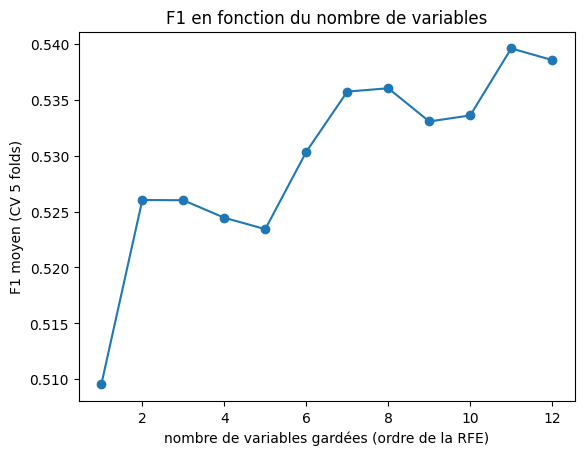
\includegraphics[width=0.55\linewidth]{f1_nb_variables.png}
\caption{Score $\Fun$ moyen (validation croisée, régression logistique) selon le nombre de variables retenues dans l'ordre de la RFE.}
\label{fig:nbvar}
\end{figure}

% ============================ 8. Modèles ==============================
\section{Modèles}\label{sec:modeles}

Les cinq modèles demandés couvrent des hypothèses très différentes, ce qui rend leur comparaison informative. On note $\mathbf{x}\in\mathbb{R}^{p}$ le vecteur des variables standardisées et $y\in\{0,1\}$ la classe.

\paragraph{Régression logistique.} Modèle linéaire probabiliste :
\begin{equation}
P(y=1 \mid \mathbf{x}) = \sigma(\mathbf{w}^\top\mathbf{x} + b), \qquad \sigma(z) = \frac{1}{1+e^{-z}}.
\end{equation}
Les paramètres minimisent l'entropie croisée binaire, éventuellement pondérée par $w_c$, augmentée d'une pénalité $\ell_2$ (Ridge) dont la force est inversement proportionnelle à l'hyperparamètre $C$ :
\begin{equation}
\min_{\mathbf{w},b}\; \frac{1}{2}\|\mathbf{w}\|_2^2 \;-\; C\sum_{i=1}^{n} w_{y_i}\Big[y_i\log \hat p_i + (1-y_i)\log(1-\hat p_i)\Big].
\end{equation}
La frontière de décision est un hyperplan : le modèle est simple et interprétable, mais exposé au \emph{biais} si la séparation réelle est non linéaire.

\paragraph{$k$ plus proches voisins ($k$-NN).} Méthode non paramétrique : un vin est classé selon le vote majoritaire de ses $k$ plus proches voisins dans l'ensemble d'apprentissage, pour la distance de Minkowski
\begin{equation}
d_p(\mathbf{x},\mathbf{x}') = \Big(\sum_{j=1}^{p}|x_j - x'_j|^{p}\Big)^{1/p},
\end{equation}
avec $p=1$ (Manhattan) ou $p=2$ (euclidienne). La complexité diminue quand $k$ augmente : un petit $k$ entraîne une forte variance. La méthode est sensible à l'échelle (d'où la standardisation) et, n'admettant pas de pondération des classes, au déséquilibre.

\paragraph{Arbre de décision.} L'espace est partitionné récursivement par des tests de la forme $x_j \leq s$. À chaque nœud, le test retenu maximise le gain d'information (critère des algorithmes ID3/C4.5), c'est-à-dire la diminution d'entropie :
\begin{equation}
H(D) = -\sum_{c} p_c \log_2 p_c, \qquad
\mathrm{Gain}(D, T) = H(D) - \sum_{v}\frac{|D_v|}{|D|}\,H(D_v).
\end{equation}
L'arbre est interprétable et insensible à l'échelle. Non contraint, il peut cependant isoler chaque exemple dans une feuille pure : il sur-apprend.

\paragraph{Naive Bayes gaussien.} Par le théorème de Bayes et sous l'hypothèse d'indépendance conditionnelle des variables,
\begin{equation}
P(y=c \mid \mathbf{x}) \;\propto\; P(y=c)\prod_{j=1}^{p}\mathcal{N}\big(x_j;\,\mu_{jc},\sigma^2_{jc}\big).
\end{equation}
Le modèle est très rapide et peu sujet au sur-apprentissage, mais ses deux hypothèses (gaussianité, indépendance) sont violées ici (section~\ref{sec:eda}).

\paragraph{Machine à vecteurs de support (SVM).} Le SVM à marge souple cherche l'hyperplan de marge maximale en tolérant des erreurs via des variables d'écart $\xi_i$ :
\begin{equation}
\min_{\mathbf{w},b,\boldsymbol{\xi}}\; \frac{1}{2}\|\mathbf{w}\|^2 + C\sum_{i=1}^{n} w_{y_i}\,\xi_i
\quad\text{s.c.}\quad \tilde y_i\big(\mathbf{w}^\top\phi(\mathbf{x}_i)+b\big) \geq 1-\xi_i,\;\; \xi_i\geq 0,
\end{equation}
avec $\tilde y_i\in\{-1,+1\}$. Le noyau gaussien (RBF) $K(\mathbf{x},\mathbf{x}') = \exp\!\big(-\gamma\|\mathbf{x}-\mathbf{x}'\|^2\big)$ permet une frontière non linéaire. $C$ règle le compromis entre largeur de marge et erreurs d'apprentissage, $\gamma$ la portée de l'influence de chaque exemple ; de grandes valeurs de l'un ou l'autre augmentent le risque de sur-apprentissage.

\paragraph{Configuration par défaut.} Les modèles sont d'abord évalués avec les paramètres par défaut de scikit-learn~\cite{pedregosa2011}, en ajoutant \code{class\_weight="balanced"} pour la régression logistique, l'arbre et le SVM, et \code{criterion="entropy"} pour l'arbre.

% ============================ 9. Évaluation ===========================
\section{Évaluation des modèles par validation croisée}\label{sec:evaluation}

\subsection{Métriques}
Avec la classe \og bon \fg{} comme classe positive, on note $TP$, $FP$, $TN$, $FN$ les effectifs de la matrice de confusion. Les métriques utilisées sont :
\begin{align}
\text{Exactitude} &= \frac{TP+TN}{TP+TN+FP+FN}, &
\text{Précision} &= \frac{TP}{TP+FP}, \\
\text{Rappel} &= \frac{TP}{TP+FN}, &
\Fun &= \frac{2\cdot\text{Précision}\cdot\text{Rappel}}{\text{Précision}+\text{Rappel}}.
\end{align}
L'AUC est l'aire sous la courbe ROC (taux de vrais positifs en fonction du taux de faux positifs, pour tous les seuils de décision). Elle s'interprète comme la probabilité qu'un bon vin tiré au hasard reçoive un score supérieur à celui d'un vin non bon tiré au hasard (0,5 : hasard ; 1 : classement parfait).

\subsection{Résultats des modèles par défaut}
Le tableau~\ref{tab:defaut} rapporte les performances hors-pli sur l'ensemble d'apprentissage.

\begin{table}[H]
\centering
\caption{Performances des modèles par défaut (validation croisée 5 plis, prédictions hors-pli sur l'apprentissage). Le $\Fun$ train est mesuré après réapprentissage sur tout l'ensemble d'apprentissage.}
\label{tab:defaut}
\small
\begin{tabular}{lcccccc}
\toprule
\textbf{Modèle} & \textbf{Exactitude} & \textbf{Précision} & \textbf{Rappel} & $\boldsymbol{\Fun}$ & \textbf{AUC} & $\boldsymbol{\Fun}$ \textbf{train} \\
\midrule
Régression logistique & 0,742 & 0,407 & 0,793 & 0,538 & 0,832 & 0,537 \\
$k$-NN ($k=5$)        & \textbf{0,820} & \textbf{0,533} & 0,410 & 0,464 & 0,786 & 0,645 \\
Arbre de décision     & 0,776 & 0,409 & 0,403 & 0,406 & 0,633 & 1,000 \\
Naive Bayes           & 0,741 & 0,392 & 0,664 & 0,493 & 0,776 & 0,496 \\
SVM (RBF)             & 0,745 & 0,412 & \textbf{0,804} & \textbf{0,545} & \textbf{0,844} & 0,577 \\
\bottomrule
\end{tabular}
\end{table}

Le SVM obtient le meilleur $\Fun$ et la meilleure AUC, suivi de près par la régression logistique. Le $k$-NN illustre le piège de l'exactitude : il obtient la meilleure exactitude (0,820) mais ne retrouve que 41\,\% des bons vins. L'arbre non contraint est le moins bon ($\Fun = 0{,}41$, AUC $= 0{,}63$).

\paragraph{Matrices de confusion.} La figure~\ref{fig:confcv} fait apparaître deux comportements. La régression logistique et le SVM, pondérés, retrouvent environ 80\,\% des 807 bons vins (640 et 649), au prix de plus de 900 fausses alertes. Le $k$-NN et l'arbre sont plus conservateurs (respectivement 290 et 470 fausses alertes) mais manquent environ 60\,\% des bons vins. Le choix entre ces profils dépend de l'usage : un caviste privilégierait la précision, un sélectionneur souhaitant ne manquer aucun bon vin privilégierait le rappel.

\begin{figure}[H]
\centering
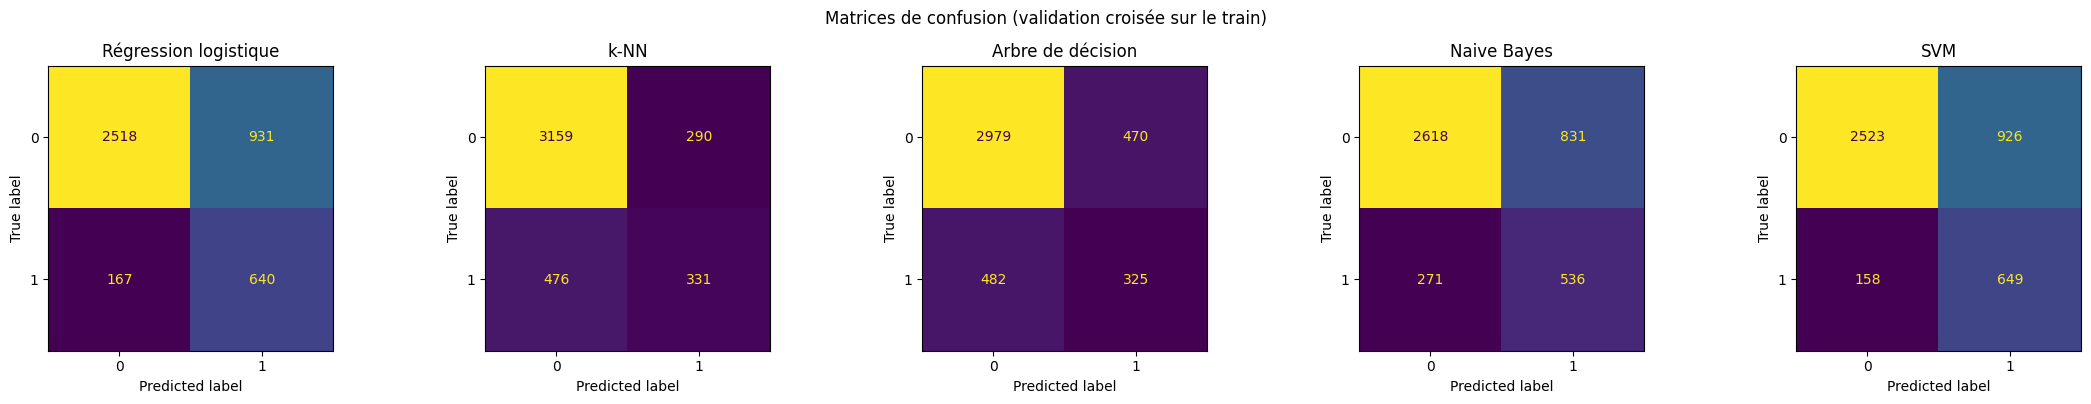
\includegraphics[width=\linewidth]{confusion_cv.png}
\caption{Matrices de confusion hors-pli des modèles par défaut (lignes : classe réelle ; colonnes : classe prédite).}
\label{fig:confcv}
\end{figure}

\paragraph{Courbes ROC.} La courbe du SVM domine, celle de la régression logistique est très proche (figure~\ref{fig:roccv}). La courbe de l'arbre présente un unique coude : ses feuilles pures ne produisent que des probabilités 0 ou 1, ce qui est un symptôme de sur-apprentissage.

\begin{figure}[H]
\centering
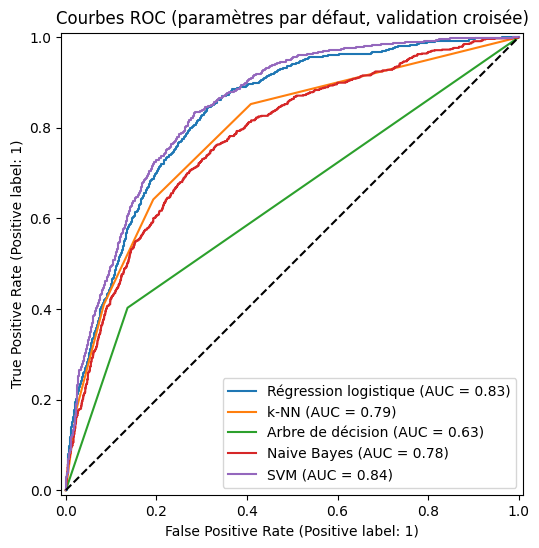
\includegraphics[width=0.48\linewidth]{roc_cv.png}
\caption{Courbes ROC hors-pli des modèles par défaut.}
\label{fig:roccv}
\end{figure}

\subsection{Diagnostic biais / variance}
L'erreur de généralisation se décompose en biais, variance et erreur irréductible. Le biais correspond à un modèle trop simple, qui se trompe sur l'apprentissage comme en validation (sous-apprentissage). La variance correspond à un modèle trop sensible aux données d'apprentissage, très performant sur celles-ci mais beaucoup moins sur des données nouvelles (sur-apprentissage). Nous comparons donc le $\Fun$ sur l'apprentissage et le $\Fun$ en validation croisée (tableau~\ref{tab:biaisvar}).

\begin{table}[H]
\centering
\caption{Diagnostic biais/variance (modèles par défaut). Le $\Fun$ de validation est la moyenne des 5 plis.}
\label{tab:biaisvar}
\small
\begin{tabular}{lccccl}
\toprule
\textbf{Modèle} & $\boldsymbol{\Fun}$ \textbf{train} & $\boldsymbol{\Fun}$ \textbf{validation} & \textbf{Écart-type} & \textbf{Écart} & \textbf{Diagnostic} \\
\midrule
Régression logistique & 0,537 & 0,539 & 0,026 & $-0{,}002$ & biais \\
$k$-NN                & 0,645 & 0,464 & 0,007 & 0,181 & variance \\
Arbre de décision     & 1,000 & 0,405 & 0,024 & 0,595 & forte variance \\
Naive Bayes           & 0,496 & 0,493 & 0,013 & 0,003 & biais \\
SVM (RBF)             & 0,577 & 0,545 & 0,017 & 0,032 & bon compromis \\
\bottomrule
\end{tabular}
\end{table}

La régression logistique et Naive Bayes présentent des scores d'apprentissage et de validation quasi identiques mais modestes : leur limite est structurelle (frontière linéaire, hypothèses trop fortes), ce qui relève du biais. L'arbre atteint $\Fun = 1$ en apprentissage mais seulement 0,405 en validation : il a mémorisé l'ensemble d'apprentissage. Le SVM combine le meilleur score de validation et un faible écart.

\paragraph{Courbes de complexité.} Pour les deux modèles dont la complexité se règle par un unique paramètre, nous traçons le $\Fun$ d'apprentissage et de validation en fonction de cette complexité (figure~\ref{fig:complexite}). Pour l'arbre, le $\Fun$ d'apprentissage croît vers 1 avec la profondeur tandis que celui de validation décroît : l'optimum est atteint pour une profondeur de 3 ($\Fun = 0{,}511$). On retrouve la forme classique de l'erreur en fonction de la complexité, avec une zone de biais à gauche et une zone de variance à droite. Pour le $k$-NN, le $\Fun$ de validation \emph{diminue} quand $k$ augmente. Sans pondération, un grand nombre de voisins fait presque toujours l'emporter la classe majoritaire, et le modèle détecte de moins en moins de bons vins. Le $k$-NN est ainsi pris entre la variance (petit $k$) et l'effet du déséquilibre (grand $k$).

\begin{figure}[H]
\centering
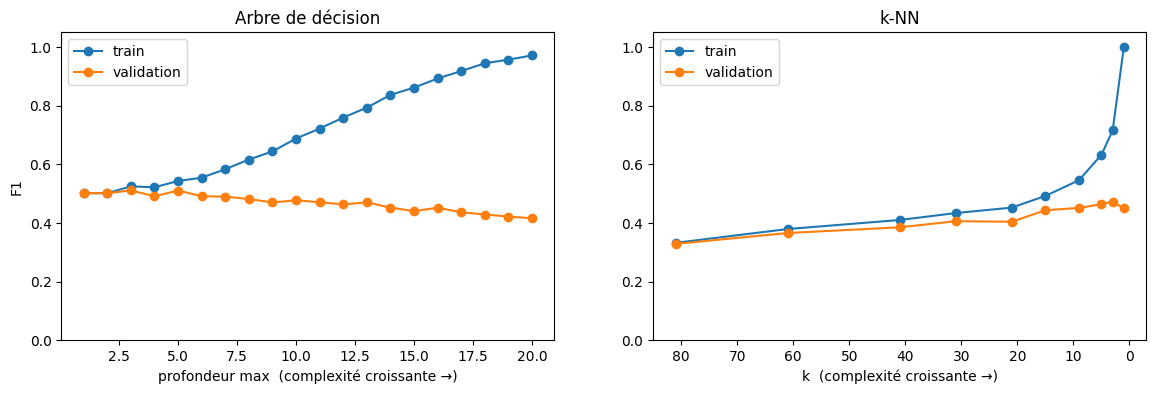
\includegraphics[width=\linewidth]{complexite.png}
\caption{$\Fun$ d'apprentissage et de validation selon la complexité : profondeur maximale de l'arbre (gauche) et nombre de voisins $k$ du $k$-NN, axe inversé (droite).}
\label{fig:complexite}
\end{figure}

% ==================== 10. Optimisation des hyperparamètres ===================
\section{Optimisation des hyperparamètres}\label{sec:optimisation}

\subsection{Méthodologie}
Les hyperparamètres, fixés avant l'apprentissage, contrôlent pour la plupart la complexité des modèles, donc le compromis biais/variance diagnostiqué ci-dessus. Deux stratégies sont employées, chaque configuration étant évaluée par validation croisée à 5 plis sur l'apprentissage avec le $\Fun$ comme critère :
\begin{itemize}
  \item la \textbf{recherche en grille} (\code{GridSearchCV}), exhaustive, adaptée lorsque l'espace de recherche est petit ;
  \item la \textbf{recherche aléatoire} (\code{RandomizedSearchCV}), qui tire un nombre fixé de configurations et réduit le coût de calcul lorsque l'espace est grand ou le modèle coûteux.
\end{itemize}
Le choix du $\Fun$ comme critère est essentiel : optimiser l'exactitude pousserait vers des modèles prédisant systématiquement la classe majoritaire. Le tableau~\ref{tab:espaces} détaille les espaces explorés. La recherche en grille est utilisée pour la régression logistique et l'arbre, dont les grilles sont petites, et la recherche aléatoire pour le SVM, modèle le plus coûteux à entraîner. Les deux stratégies sont appliquées au $k$-NN afin de les comparer. Naive Bayes gaussien n'est pas optimisé : il ne possède pas d'hyperparamètre structurant, ses seuls paramètres (moyennes et variances par classe) étant estimés à partir des données.

\begin{table}[H]
\centering
\caption{Espaces de recherche des hyperparamètres.}
\label{tab:espaces}
\small
\resizebox{\linewidth}{!}{%
\begin{tabular}{llll}
\toprule
\textbf{Modèle} & \textbf{Méthode} & \textbf{Espace de recherche} & \textbf{Configurations} \\
\midrule
Régression logistique & grille & $C\in\{10^{-3},\dots,10^{2}\}$, \code{class\_weight} $\in\{\text{aucun}, \text{balanced}\}$ & 12 \\
Arbre (entropie) & grille & \makecell[l]{profondeur $\in\{3,5,7,10,15,\infty\}$,\\ taille min. des feuilles $\in\{1,5,10,20,50\}$, \code{class\_weight}} & 60 \\
\multirow{2}{*}{$k$-NN} & grille & $k\in\{1,3,5,7,9,11,15,21,31\}$, $p\in\{1,2\}$ & 18 \\
 & aléatoire & $k\in\{1,\dots,39\}$, $p\in\{1,2\}$ & 10 tirées sur 78 \\
SVM (RBF) & aléatoire & \makecell[l]{$C\in\{0{,}1;\,0{,}3;\,1;\,3;\,10;\,30;\,100\}$,\\ $\gamma\in\{0{,}001;\,0{,}003;\,\dots;\,1\}$} & 20 tirées sur 49 \\
\bottomrule
\end{tabular}}
\end{table}

\subsection{Résultats}

\begin{table}[H]
\centering
\caption{Hyperparamètres retenus et $\Fun$ moyen en validation croisée avant et après optimisation.}
\label{tab:optim}
\small
\begin{tabular}{llcc}
\toprule
\textbf{Modèle} & \textbf{Configuration retenue} & $\boldsymbol{\Fun}$ \textbf{défaut} & $\boldsymbol{\Fun}$ \textbf{optimisé} \\
\midrule
Régression logistique & $C=0{,}01$, balanced & 0,539 & 0,540 \\
Arbre de décision     & profondeur 3, feuille min. 1, balanced & 0,405 & \textbf{0,511} \\
$k$-NN                & $k=1$, Manhattan ($p=1$) & 0,464 & 0,482 \\
Naive Bayes           & -- & 0,493 & 0,493 \\
SVM (RBF)             & $C=100$, $\gamma=0{,}01$, balanced & \textbf{0,545} & \textbf{0,544} \\
\bottomrule
\end{tabular}
\end{table}

L'\textbf{arbre} est le modèle qui bénéficie le plus de l'optimisation ($+0{,}11$). La profondeur retenue (3) coïncide avec l'optimum de la courbe de complexité : limiter la profondeur supprime l'essentiel de la variance. La \textbf{régression logistique} ne progresse pratiquement pas malgré une régularisation forte ($C=0{,}01$), ce qui confirme que sa limite est un biais structurel. Pour le \textbf{SVM}, la configuration trouvée égale la configuration par défaut ($\gamma=\texttt{scale}=1/p\approx0{,}083$ sur données standardisées, $C=1$) : celle-ci se situait déjà dans une zone favorable. Pour le \textbf{$k$-NN}, les deux recherches aboutissent à la même configuration ($k=1$, distance de Manhattan), la recherche aléatoire avec presque deux fois moins d'évaluations. Ce résultat appelle toutefois une réserve : $k=1$ est le cas de variance maximale. Le critère $\Fun$ favorise les petites valeurs de $k$ parce qu'en l'absence de pondération, c'est la seule manière pour le $k$-NN de prédire suffisamment de bons vins. Enfin, la pondération \code{balanced} est retenue pour la régression logistique comme pour l'arbre, ce qui confirme la nécessité de traiter le déséquilibre.

\begin{figure}[H]
\centering
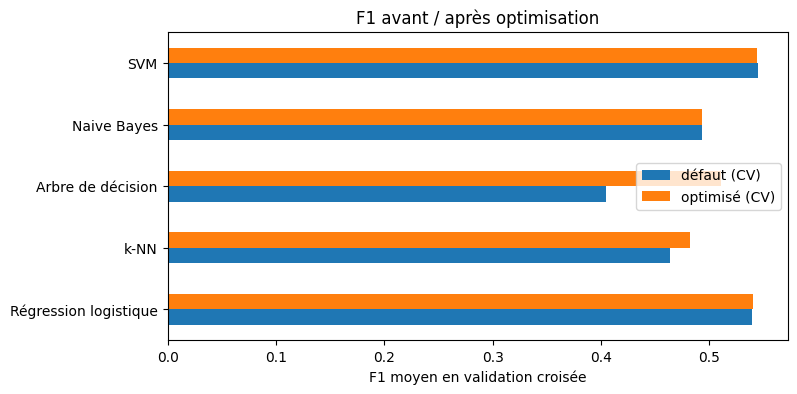
\includegraphics[width=0.62\linewidth]{f1_avant_apres.png}
\caption{$\Fun$ moyen en validation croisée avant et après optimisation.}
\label{fig:avantapres}
\end{figure}

% ======================== 11. Évaluation finale ========================
\section{Évaluation finale sur le jeu de test}\label{sec:final}

Le modèle final est choisi sur la base du $\Fun$ en validation croisée, \emph{avant} toute utilisation du test. Les cinq modèles optimisés sont ensuite réentraînés sur l'ensemble d'apprentissage complet et évalués une seule fois sur le test (tableau~\ref{tab:test}).

\begin{table}[H]
\centering
\caption{Évaluation finale des modèles optimisés sur le jeu de test (1\,064 vins, dont 202 bons), triés par $\Fun$ de validation croisée.}
\label{tab:test}
\small
\begin{tabular}{lccccccc}
\toprule
\textbf{Modèle} & $\boldsymbol{\Fun}$ \textbf{CV} & \textbf{Exactitude} & \textbf{Précision} & \textbf{Rappel} & $\boldsymbol{\Fun}$ \textbf{test} & \textbf{AUC} & $\boldsymbol{\Fun}$ \textbf{train} \\
\midrule
SVM (RBF)             & \textbf{0,544} & 0,736 & 0,403 & \textbf{0,817} & \textbf{0,540} & \textbf{0,850} & 0,573 \\
Régression logistique & 0,540 & 0,735 & 0,400 & 0,797 & 0,533 & 0,817 & 0,541 \\
Arbre de décision     & 0,511 & 0,709 & 0,366 & 0,733 & 0,488 & 0,791 & 0,525 \\
Naive Bayes           & 0,493 & 0,733 & 0,382 & 0,653 & 0,482 & 0,759 & 0,496 \\
$k$-NN                & 0,482 & \textbf{0,822} & \textbf{0,532} & 0,540 & 0,536 & 0,714 & 1,000 \\
\bottomrule
\end{tabular}
\end{table}

Pour le SVM, la régression logistique et Naive Bayes, les scores de test sont très proches des scores de validation croisée (écarts inférieurs à 0,012), ce qui atteste de la fiabilité du protocole. Le $k$-NN obtient un $\Fun$ de test (0,536) nettement supérieur à son $\Fun$ de validation (0,482). Associé à la plus faible AUC (0,714) et à un $\Fun$ d'apprentissage de 1, ce résultat relève vraisemblablement de la variabilité d'échantillonnage. Il ne peut de toute façon pas servir à choisir le modèle sans réutiliser le test.

Le \textbf{SVM à noyau RBF} est retenu comme modèle final : il est le meilleur en validation croisée comme sur le test ($\Fun = 0{,}540$, AUC $= 0{,}850$) et présente le meilleur compromis biais/variance. Sur le test, il retrouve 165 des 202 bons vins (rappel de 82\,\%), au prix de 244 fausses alertes sur 862 vins non bons (précision de 40\,\%), comme le montre la figure~\ref{fig:final}.

\begin{figure}[H]
\centering
\begin{subfigure}[b]{0.44\linewidth}
  \centering
  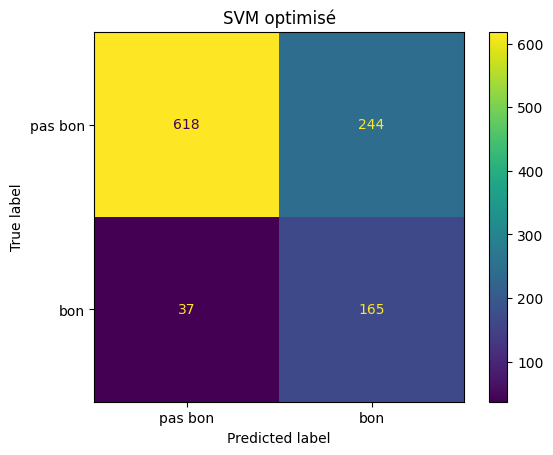
\includegraphics[width=\linewidth]{confusion_svm_test.png}
  \caption{Matrice de confusion du SVM.}
\end{subfigure}
\hfill
\begin{subfigure}[b]{0.44\linewidth}
  \centering
  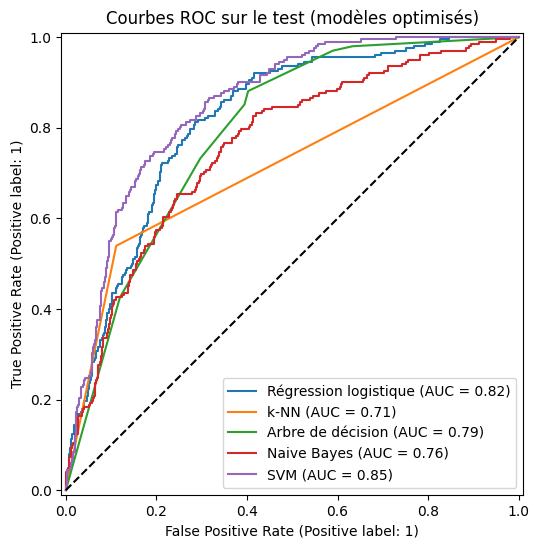
\includegraphics[width=\linewidth]{roc_test.png}
  \caption{Courbes ROC des modèles optimisés.}
\end{subfigure}
\caption{Évaluation finale sur le jeu de test.}
\label{fig:final}
\end{figure}

\paragraph{Interprétation géométrique.} Pour visualiser le comportement du SVM, un modèle de mêmes hyperparamètres est entraîné sur les deux variables les mieux classées par la RFE, l'alcool et l'acidité volatile (figure~\ref{fig:frontiere}). Il s'agit d'une illustration et non du modèle final, qui utilise les douze variables. Quatre observations ressortent :
\begin{itemize}
  \item les bons vins se concentrent dans la région \og alcool élevé, acidité volatile faible à modérée \fg{} ;
  \item la frontière est courbe et oblique : plus l'acidité volatile est élevée, plus la teneur en alcool requise pour être classé \og bon \fg{} augmente, ce qu'un modèle linéaire ne peut pas représenter ;
  \item les deux classes se chevauchent largement, ce qui borne les performances atteignables ;
  \item la région \og bon \fg{} est étendue du fait de la pondération des classes, ce qui explique le rappel élevé et la précision modeste.
\end{itemize}

\begin{figure}[H]
\centering
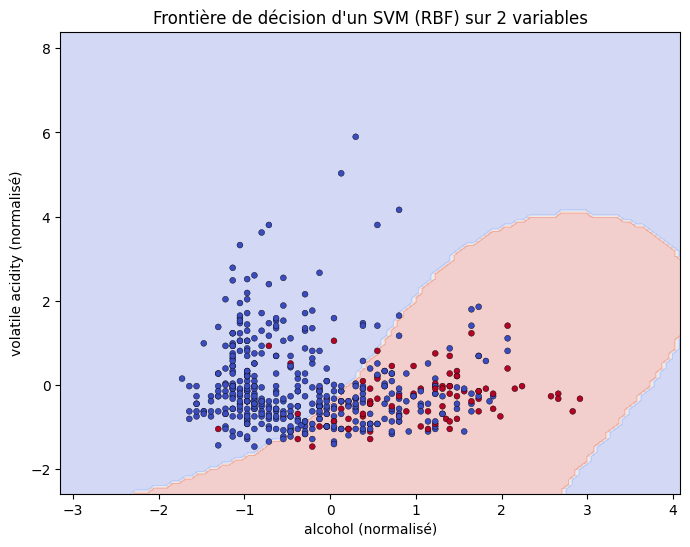
\includegraphics[width=0.6\linewidth]{svm_frontiere.png}
\caption{Frontière de décision d'un SVM RBF ($C=100$, $\gamma=0{,}01$) entraîné sur l'alcool et l'acidité volatile (variables standardisées). Zone rouge : prédiction \og bon \fg{}. Points : 500 vins de l'apprentissage.}
\label{fig:frontiere}
\end{figure}

% ============================ 12. Discussion ===========================
\section{Discussion}\label{sec:discussion}

\paragraph{Niveau de performance.} Un $\Fun$ de 0,54 peut paraître modeste. Plusieurs facteurs l'expliquent. La note est une médiane d'appréciations subjectives, et la frontière à 7 sépare des vins (notés 6 et 7) souvent très proches chimiquement. Les variables disponibles ne décrivent pas tous les déterminants de la qualité : cépage, millésime, arômes ou prix n'y figurent pas. Enfin, la figure~\ref{fig:frontiere} montre un recouvrement important des classes. L'AUC de 0,85 indique néanmoins que le modèle ordonne correctement les vins dans la grande majorité des cas.

\paragraph{Compromis précision/rappel.} Le modèle final privilégie le rappel. Ce compromis découle de la pondération des classes et du seuil de décision par défaut. Selon l'usage (recommandation à un client contre présélection pour une dégustation), un autre point de fonctionnement sur la courbe ROC pourrait être préférable. Ajuster le seuil par validation croisée constitue d'ailleurs une alternative à la pondération des classes, applicable aux cinq modèles, y compris le $k$-NN et Naive Bayes qui n'admettent pas \code{class\_weight}.

\paragraph{Limites méthodologiques.}
\begin{itemize}
  \item La standardisation est ajustée sur l'ensemble d'apprentissage complet avant la validation croisée. Chaque pli de validation contribue donc marginalement au calcul des moyennes et écarts-types. L'effet est négligeable ici, mais l'usage d'un \code{Pipeline} scikit-learn l'éliminerait.
  \item La RFE repose sur un modèle linéaire. Une sélection fondée sur un modèle non linéaire pourrait produire un classement différent.
  \item Les performances proviennent d'un unique découpage apprentissage/test. Une validation croisée répétée ou imbriquée fournirait des intervalles de confiance plus fiables, en particulier pour départager le SVM et la régression logistique, dont les scores diffèrent de moins d'un écart-type.
  \item La binarisation au seuil 7 fait perdre l'information ordinale de la note.
\end{itemize}

\paragraph{Perspectives.} Plusieurs pistes peuvent être explorées :
\begin{itemize}
  \item les méthodes d'ensemble : forêts aléatoires (\emph{bagging}), AdaBoost (\emph{boosting}) ou empilement (\emph{stacking}) des modèles étudiés, généralement plus performantes que les modèles individuels sur ce type de données tabulaires ;
  \item l'ajustement du seuil de décision à partir de la courbe ROC ;
  \item des modèles distincts pour les vins rouges et blancs ;
  \item une formulation en régression ou en classification ordinale exploitant la note complète.
\end{itemize}

% ============================ 13. Conclusion ===========================
\section{Conclusion}

Ce projet a mis en œuvre une chaîne complète d'apprentissage supervisé pour prédire la qualité d'un vin à partir de mesures physico-chimiques. Le déséquilibre des classes (19\,\% de bons vins) a structuré les choix méthodologiques : découpage stratifié, pondération des classes, score $\Fun$ et AUC comme critères. L'analyse exploratoire et la sélection par RFE convergent sur le rôle prépondérant du degré d'alcool et de l'acidité volatile. La comparaison des cinq modèles, menée exclusivement par validation croisée, a permis d'identifier les sources d'erreur de chacun : biais pour la régression logistique et Naive Bayes, variance pour l'arbre non contraint et le $k$-NN. L'optimisation des hyperparamètres a surtout bénéficié à l'arbre, dont la profondeur limitée corrige le sur-apprentissage. Évalué une seule fois sur le jeu de test, le SVM à noyau RBF obtient les meilleures performances ($\Fun = 0{,}54$, AUC $= 0{,}85$, rappel $= 0{,}82$), avec un écart minime entre validation et test. Ses performances restent néanmoins limitées par la subjectivité de la note et le recouvrement des classes. Les méthodes d'ensemble et l'ajustement du seuil de décision constituent les prolongements les plus prometteurs.

% ============================ Références ===============================
\begin{thebibliography}{9}
\bibitem{cortez2009}
P.~Cortez, A.~Cerdeira, F.~Almeida, T.~Matos et J.~Reis.
\newblock Modeling wine preferences by data mining from physicochemical properties.
\newblock \emph{Decision Support Systems}, 47(4):547--553, 2009.

\bibitem{pedregosa2011}
F.~Pedregosa \emph{et al.}
\newblock Scikit-learn: Machine learning in Python.
\newblock \emph{Journal of Machine Learning Research}, 12:2825--2830, 2011.

\bibitem{tukey1977}
J.~W.~Tukey.
\newblock \emph{Exploratory Data Analysis}.
\newblock Addison-Wesley, 1977.

\bibitem{cours}
A.~G.~Blaiech, A.~Tay et H.~Shraim.
\newblock \emph{Cours de Machine Learning I}, chapitres I à VI.
\newblock EFREI Paris, 2026--2027.
\end{thebibliography}

% ============================== Annexe =================================
\appendix
\section{Reproductibilité}
L'ensemble des traitements est contenu dans le notebook \code{projet\_vin.ipynb} (Python, pandas, scikit-learn, matplotlib, seaborn). Les sources d'aléa sont fixées (\code{random\_state=42}) pour le découpage, l'arbre, le SVM et les recherches aléatoires. Les validations croisées utilisent un découpage stratifié à 5 plis (\code{cv=5}). Les fichiers \code{winequality-red.csv} et \code{winequality-white.csv} doivent être placés dans le dossier \code{data/} du dépôt.

\end{document}
